\documentclass[1p]{elsarticle_modified}
%\bibliographystyle{elsarticle-num}

%\usepackage[colorlinks]{hyperref}
%\usepackage{abbrmath_seonhwa} %\Abb, \Ascr, \Acal ,\Abf, \Afrak
\usepackage{amsfonts}
\usepackage{amssymb}
\usepackage{amsmath}
\usepackage{amsthm}
\usepackage{scalefnt}
\usepackage{amsbsy}
\usepackage{kotex}
\usepackage{caption}
\usepackage{subfig}
\usepackage{color}
\usepackage{graphicx}
\usepackage{xcolor} %% white, black, red, green, blue, cyan, magenta, yellow
\usepackage{float}
\usepackage{setspace}
\usepackage{hyperref}

\usepackage{tikz}
\usetikzlibrary{arrows}

\usepackage{multirow}
\usepackage{array} % fixed length table
\usepackage{hhline}

%%%%%%%%%%%%%%%%%%%%%
\makeatletter
\renewcommand*\env@matrix[1][\arraystretch]{%
	\edef\arraystretch{#1}%
	\hskip -\arraycolsep
	\let\@ifnextchar\new@ifnextchar
	\array{*\c@MaxMatrixCols c}}
\makeatother %https://tex.stackexchange.com/questions/14071/how-can-i-increase-the-line-spacing-in-a-matrix
%%%%%%%%%%%%%%%

\usepackage[normalem]{ulem}

\newcommand{\msout}[1]{\ifmmode\text{\sout{\ensuremath{#1}}}\else\sout{#1}\fi}
%SOURCE: \msout is \stkout macro in https://tex.stackexchange.com/questions/20609/strikeout-in-math-mode

\newcommand{\cancel}[1]{
	\ifmmode
	{\color{red}\msout{#1}}
	\else
	{\color{red}\sout{#1}}
	\fi
}

\newcommand{\add}[1]{
	{\color{blue}\uwave{#1}}
}

\newcommand{\replace}[2]{
	\ifmmode
	{\color{red}\msout{#1}}{\color{blue}\uwave{#2}}
	\else
	{\color{red}\sout{#1}}{\color{blue}\uwave{#2}}
	\fi
}

\newcommand{\Sol}{\mathcal{S}} %segment
\newcommand{\D}{D} %diagram
\newcommand{\A}{\mathcal{A}} %arc


%%%%%%%%%%%%%%%%%%%%%%%%%%%%%5 test

\def\sl{\operatorname{\textup{SL}}(2,\Cbb)}
\def\psl{\operatorname{\textup{PSL}}(2,\Cbb)}
\def\quan{\mkern 1mu \triangleright \mkern 1mu}

\theoremstyle{definition}
\newtheorem{thm}{Theorem}[section]
\newtheorem{prop}[thm]{Proposition}
\newtheorem{lem}[thm]{Lemma}
\newtheorem{ques}[thm]{Question}
\newtheorem{cor}[thm]{Corollary}
\newtheorem{defn}[thm]{Definition}
\newtheorem{exam}[thm]{Example}
\newtheorem{rmk}[thm]{Remark}
\newtheorem{alg}[thm]{Algorithm}

\newcommand{\I}{\sqrt{-1}}
\begin{document}

%\begin{frontmatter}
%
%\title{Boundary parabolic representations of knots up to 8 crossings}
%
%%% Group authors per affiliation:
%\author{Yunhi Cho} 
%\address{Department of Mathematics, University of Seoul, Seoul, Korea}
%\ead{yhcho@uos.ac.kr}
%
%
%\author{Seonhwa Kim} %\fnref{s_kim}}
%\address{Center for Geometry and Physics, Institute for Basic Science, Pohang, 37673, Korea}
%\ead{ryeona17@ibs.re.kr}
%
%\author{Hyuk Kim}
%\address{Department of Mathematical Sciences, Seoul National University, Seoul 08826, Korea}
%\ead{hyukkim@snu.ac.kr}
%
%\author{Seokbeom Yoon}
%\address{Department of Mathematical Sciences, Seoul National University, Seoul, 08826,  Korea}
%\ead{sbyoon15@snu.ac.kr}
%
%\begin{abstract}
%We find all boundary parabolic representation of knots up to 8 crossings.
%
%\end{abstract}
%\begin{keyword}
%    \MSC[2010] 57M25 
%\end{keyword}
%
%\end{frontmatter}

%\linenumbers
%\tableofcontents
%
\newcommand\colored[1]{\textcolor{white}{\rule[-0.35ex]{0.8em}{1.4ex}}\kern-0.8em\color{red} #1}%
%\newcommand\colored[1]{\textcolor{white}{ #1}\kern-2.17ex	\textcolor{white}{ #1}\kern-1.81ex	\textcolor{white}{ #1}\kern-2.15ex\color{red}#1	}

{\Large $\underline{11n_{149}~(K11n_{149})}$}

\setlength{\tabcolsep}{10pt}
\renewcommand{\arraystretch}{1.6}
\vspace{1cm}\begin{tabular}{m{100pt}>{\centering\arraybackslash}m{274pt}}
\multirow{5}{120pt}{
	\centering
	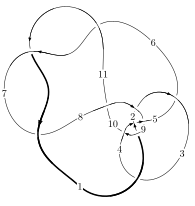
\includegraphics[width=112pt]{../../../GIT/diagram.site/Diagrams/png/765_11n_149.png}\\
\ \ \ A knot diagram\footnotemark}&
\allowdisplaybreaks
\textbf{Linearized knot diagam} \\
\cline{2-2}
 &
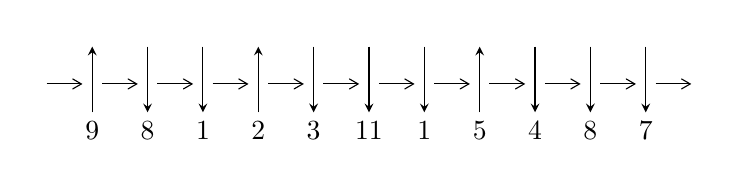
\begin{tikzpicture}[x=20pt, y=17pt]
	% nodes
	\node (C0) at (0, 0) {};
	\node (C1) at (1, 0) {};
	\node (C1U) at (1, +1) {};
	\node (C1D) at (1, -1) {9};

	\node (C2) at (2, 0) {};
	\node (C2U) at (2, +1) {};
	\node (C2D) at (2, -1) {8};

	\node (C3) at (3, 0) {};
	\node (C3U) at (3, +1) {};
	\node (C3D) at (3, -1) {1};

	\node (C4) at (4, 0) {};
	\node (C4U) at (4, +1) {};
	\node (C4D) at (4, -1) {2};

	\node (C5) at (5, 0) {};
	\node (C5U) at (5, +1) {};
	\node (C5D) at (5, -1) {3};

	\node (C6) at (6, 0) {};
	\node (C6U) at (6, +1) {};
	\node (C6D) at (6, -1) {11};

	\node (C7) at (7, 0) {};
	\node (C7U) at (7, +1) {};
	\node (C7D) at (7, -1) {1};

	\node (C8) at (8, 0) {};
	\node (C8U) at (8, +1) {};
	\node (C8D) at (8, -1) {5};

	\node (C9) at (9, 0) {};
	\node (C9U) at (9, +1) {};
	\node (C9D) at (9, -1) {4};

	\node (C10) at (10, 0) {};
	\node (C10U) at (10, +1) {};
	\node (C10D) at (10, -1) {8};

	\node (C11) at (11, 0) {};
	\node (C11U) at (11, +1) {};
	\node (C11D) at (11, -1) {7};
	\node (C12) at (12, 0) {};

	% arrows
	\draw[->,>={angle 60}]
	(C0) edge (C1) (C1) edge (C2) (C2) edge (C3) (C3) edge (C4) (C4) edge (C5) (C5) edge (C6) (C6) edge (C7) (C7) edge (C8) (C8) edge (C9) (C9) edge (C10) (C10) edge (C11) (C11) edge (C12) ;	\draw[->,>=stealth]
	(C1D) edge (C1U) (C2U) edge (C2D) (C3U) edge (C3D) (C4D) edge (C4U) (C5U) edge (C5D) (C6U) edge (C6D) (C7U) edge (C7D) (C8D) edge (C8U) (C9U) edge (C9D) (C10U) edge (C10D) (C11U) edge (C11D) ;
	\end{tikzpicture} \\
\hhline{~~} \\& 
\textbf{Solving Sequence} \\ \cline{2-2} 
 &
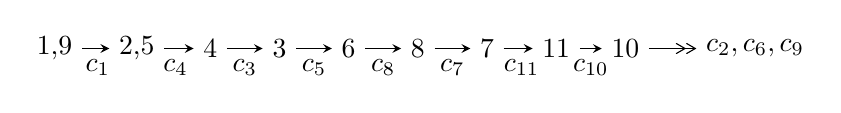
\begin{tikzpicture}[x=25pt, y=7pt]
	% node
	\node (A0) at (-1/8, 0) {1,9};
	\node (A1) at (17/16, 0) {2,5};
	\node (A2) at (17/8, 0) {4};
	\node (A3) at (25/8, 0) {3};
	\node (A4) at (33/8, 0) {6};
	\node (A5) at (41/8, 0) {8};
	\node (A6) at (49/8, 0) {7};
	\node (A7) at (57/8, 0) {11};
	\node (A8) at (65/8, 0) {10};
	\node (C1) at (1/2, -1) {$c_{1}$};
	\node (C2) at (13/8, -1) {$c_{4}$};
	\node (C3) at (21/8, -1) {$c_{3}$};
	\node (C4) at (29/8, -1) {$c_{5}$};
	\node (C5) at (37/8, -1) {$c_{8}$};
	\node (C6) at (45/8, -1) {$c_{7}$};
	\node (C7) at (53/8, -1) {$c_{11}$};
	\node (C8) at (61/8, -1) {$c_{10}$};
	\node (A9) at (10, 0) {$c_{2},c_{6},c_{9}$};

	% edge
	\draw[->,>=stealth]	
	(A0) edge (A1) (A1) edge (A2) (A2) edge (A3) (A3) edge (A4) (A4) edge (A5) (A5) edge (A6) (A6) edge (A7) (A7) edge (A8) ;
	\draw[->>,>={angle 60}]	
	(A8) edge (A9);
\end{tikzpicture} \\ 

\end{tabular} \\

\footnotetext{
The image of knot diagram is generated by the software ``\textbf{Draw programme}" developed by Andrew Bartholomew(\url{http://www.layer8.co.uk/maths/draw/index.htm\#Running-draw}), where we modified some parts for our purpose(\url{https://github.com/CATsTAILs/LinksPainter}).
}\phantom \\ \newline 
\centering \textbf{Ideals for irreducible components\footnotemark of $X_{\text{par}}$} 
 
\begin{align*}
I^u_{1}&=\langle 
25 u^{12}-16 u^{11}+60 u^{10}+12 u^9+170 u^8+6 u^7+155 u^6+188 u^5+70 u^4+151 u^3+68 u^2+11 b+51 u+21,\\
\phantom{I^u_{1}}&\phantom{= \langle  }a-1,\;u^{13}- u^{12}+3 u^{11}- u^{10}+8 u^9-3 u^8+9 u^7+3 u^6+4 u^5+6 u^4+4 u^2+1\rangle \\
I^u_{2}&=\langle 
- u^5- u^4+b- u-1,\;a+1,\;u^7+u^6- u^4+u^3+2 u^2-1\rangle \\
I^u_{3}&=\langle 
b+1,\;-2889 u^{11}+13347 u^{10}+\cdots+24775 a+75210,\\
\phantom{I^u_{3}}&\phantom{= \langle  }u^{12}-2 u^{11}+2 u^{10}- u^9+10 u^8-16 u^7+25 u^6-16 u^5+20 u^4-9 u^3+15 u^2-3 u+5\rangle \\
I^u_{4}&=\langle 
b-1,\;a+u,\;u^2+u+1\rangle \\
\\
\end{align*}
\raggedright * 4 irreducible components of $\dim_{\mathbb{C}}=0$, with total 34 representations.\\
\footnotetext{All coefficients of polynomials are rational numbers. But the coefficients are sometimes approximated in decimal forms when there is not enough margin.}
\newpage
\renewcommand{\arraystretch}{1}
\centering \section*{I. $I^u_{1}= \langle 25 u^{12}-16 u^{11}+\cdots+11 b+21,\;a-1,\;u^{13}- u^{12}+\cdots+4 u^2+1 \rangle$}
\flushleft \textbf{(i) Arc colorings}\\
\begin{tabular}{m{7pt} m{180pt} m{7pt} m{180pt} }
\flushright $a_{1}=$&$\begin{pmatrix}1\\0\end{pmatrix}$ \\
\flushright $a_{9}=$&$\begin{pmatrix}0\\u\end{pmatrix}$ \\
\flushright $a_{2}=$&$\begin{pmatrix}1\\- u^2\end{pmatrix}$ \\
\flushright $a_{5}=$&$\begin{pmatrix}1\\-2.27273 u^{12}+1.45455 u^{11}+\cdots-4.63636 u-1.90909\end{pmatrix}$ \\
\flushright $a_{4}=$&$\begin{pmatrix}2.27273 u^{12}-1.45455 u^{11}+\cdots+4.63636 u+2.90909\\-1.72727 u^{12}+0.545455 u^{11}+\cdots-2.36364 u-1.09091\end{pmatrix}$ \\
\flushright $a_{3}=$&$\begin{pmatrix}0.545455 u^{12}-0.909091 u^{11}+\cdots+2.27273 u+1.81818\\-1.72727 u^{12}+0.545455 u^{11}+\cdots-2.36364 u-1.09091\end{pmatrix}$ \\
\flushright $a_{6}=$&$\begin{pmatrix}2.36364 u^{12}-0.272727 u^{11}+\cdots+1.18182 u+1.54545\\1.27273 u^{12}+0.545455 u^{11}+\cdots+1.63636 u+0.909091\end{pmatrix}$ \\
\flushright $a_{8}=$&$\begin{pmatrix}- u\\0.818182 u^{12}-1.36364 u^{11}+\cdots+2.90909 u-2.27273\end{pmatrix}$ \\
\flushright $a_{7}=$&$\begin{pmatrix}0.818182 u^{12}-1.36364 u^{11}+\cdots+1.90909 u-2.27273\\0.818182 u^{12}-1.36364 u^{11}+\cdots+2.90909 u-2.27273\end{pmatrix}$ \\
\flushright $a_{11}=$&$\begin{pmatrix}1.09091 u^{12}+1.18182 u^{11}+\cdots-0.454545 u+1.63636\\1.63636 u^{12}+0.272727 u^{11}+\cdots+1.81818 u+1.45455\end{pmatrix}$ \\
\flushright $a_{10}=$&$\begin{pmatrix}-0.727273 u^{12}+2.54545 u^{11}+\cdots-1.36364 u+2.90909\\-0.545455 u^{12}-0.0909091 u^{11}+\cdots-1.27273 u+1.18182\end{pmatrix}$\\ \flushright $a_{10}=$&$\begin{pmatrix}-0.727273 u^{12}+2.54545 u^{11}+\cdots-1.36364 u+2.90909\\-0.545455 u^{12}-0.0909091 u^{11}+\cdots-1.27273 u+1.18182\end{pmatrix}$\\&\end{tabular}
\flushleft \textbf{(ii) Obstruction class $= -1$}\\~\\
\flushleft \textbf{(iii) Cusp Shapes $= -\frac{76}{11} u^{12}+\frac{189}{11} u^{11}-\frac{332}{11} u^{10}+\frac{334}{11} u^9-\frac{618}{11} u^8+\frac{926}{11} u^7-\frac{898}{11} u^6+\frac{257}{11} u^5+\frac{335}{11} u^4-\frac{463}{11} u^3+\frac{415}{11} u^2-\frac{313}{11} u+\frac{18}{11}$}\\~\\
\newpage\renewcommand{\arraystretch}{1}
\flushleft \textbf{(iv) u-Polynomials at the component}\newline \\
\begin{tabular}{m{50pt}|m{274pt}}
Crossings & \hspace{64pt}u-Polynomials at each crossing \\
\hline $$\begin{aligned}c_{1},c_{8}\end{aligned}$$&$\begin{aligned}
&u^{13}- u^{12}+3 u^{11}- u^{10}+8 u^9-3 u^8+9 u^7+3 u^6+4 u^5+6 u^4+4 u^2+1
\end{aligned}$\\
\hline $$\begin{aligned}c_{2},c_{9}\end{aligned}$$&$\begin{aligned}
&u^{13}-7 u^{11}+\cdots+7 u+5
\end{aligned}$\\
\hline $$\begin{aligned}c_{3},c_{5}\end{aligned}$$&$\begin{aligned}
&u^{13}-15 u^{11}+\cdots+7 u-1
\end{aligned}$\\
\hline $$\begin{aligned}c_{4}\end{aligned}$$&$\begin{aligned}
&u^{13}+10 u^{12}+\cdots+15 u+2
\end{aligned}$\\
\hline $$\begin{aligned}c_{6},c_{7},c_{11}\end{aligned}$$&$\begin{aligned}
&u^{13}+5 u^{12}+\cdots+17 u+4
\end{aligned}$\\
\hline $$\begin{aligned}c_{10}\end{aligned}$$&$\begin{aligned}
&u^{13}-15 u^{12}+\cdots-57 u-4
\end{aligned}$\\
\hline
\end{tabular}\\~\\
\newpage\renewcommand{\arraystretch}{1}
\flushleft \textbf{(v) Riley Polynomials at the component}\newline \\
\begin{tabular}{m{50pt}|m{274pt}}
Crossings & \hspace{64pt}Riley Polynomials at each crossing \\
\hline $$\begin{aligned}c_{1},c_{8}\end{aligned}$$&$\begin{aligned}
&y^{13}+5 y^{12}+\cdots-8 y-1
\end{aligned}$\\
\hline $$\begin{aligned}c_{2},c_{9}\end{aligned}$$&$\begin{aligned}
&y^{13}-14 y^{12}+\cdots+209 y-25
\end{aligned}$\\
\hline $$\begin{aligned}c_{3},c_{5}\end{aligned}$$&$\begin{aligned}
&y^{13}-30 y^{12}+\cdots+113 y-1
\end{aligned}$\\
\hline $$\begin{aligned}c_{4}\end{aligned}$$&$\begin{aligned}
&y^{13}+28 y^{11}+\cdots-15 y-4
\end{aligned}$\\
\hline $$\begin{aligned}c_{6},c_{7},c_{11}\end{aligned}$$&$\begin{aligned}
&y^{13}-19 y^{12}+\cdots+41 y-16
\end{aligned}$\\
\hline $$\begin{aligned}c_{10}\end{aligned}$$&$\begin{aligned}
&y^{13}-55 y^{12}+\cdots+969 y-16
\end{aligned}$\\
\hline
\end{tabular}\\~\\
\newpage\flushleft \textbf{(vi) Complex Volumes and Cusp Shapes}
$$\begin{array}{c|c|c}  
\text{Solutions to }I^u_{1}& \I (\text{vol} + \sqrt{-1}CS) & \text{Cusp shape}\\
 \hline 
\begin{aligned}
u &= \phantom{-}0.674712 + 0.924636 I \\
a &= \phantom{-}1.00000\phantom{ +0.000000I} \\
b &= \phantom{-}0.661360 - 0.645036 I\end{aligned}
 & -0.51141 + 2.45131 I & -7.77475 - 3.59431 I \\ \hline\begin{aligned}
u &= \phantom{-}0.674712 - 0.924636 I \\
a &= \phantom{-}1.00000\phantom{ +0.000000I} \\
b &= \phantom{-}0.661360 + 0.645036 I\end{aligned}
 & -0.51141 - 2.45131 I & -7.77475 + 3.59431 I \\ \hline\begin{aligned}
u &= -0.846831\phantom{ +0.000000I} \\
a &= \phantom{-}1.00000\phantom{ +0.000000I} \\
b &= -0.355630\phantom{ +0.000000I}\end{aligned}
 & -1.94524\phantom{ +0.000000I} & -3.64330\phantom{ +0.000000I} \\ \hline\begin{aligned}
u &= \phantom{-}0.448030 + 0.671291 I \\
a &= \phantom{-}1.00000\phantom{ +0.000000I} \\
b &= \phantom{-}2.26733 - 1.80136 I\end{aligned}
 & -15.3014 + 1.1163 I & -12.72292 - 6.16579 I \\ \hline\begin{aligned}
u &= \phantom{-}0.448030 - 0.671291 I \\
a &= \phantom{-}1.00000\phantom{ +0.000000I} \\
b &= \phantom{-}2.26733 + 1.80136 I\end{aligned}
 & -15.3014 - 1.1163 I & -12.72292 + 6.16579 I \\ \hline\begin{aligned}
u &= -0.203954 + 0.727117 I \\
a &= \phantom{-}1.00000\phantom{ +0.000000I} \\
b &= \phantom{-}1.41448 + 1.32960 I\end{aligned}
 & -4.93091 - 1.68363 I & -14.6461 + 4.3140 I \\ \hline\begin{aligned}
u &= -0.203954 - 0.727117 I \\
a &= \phantom{-}1.00000\phantom{ +0.000000I} \\
b &= \phantom{-}1.41448 - 1.32960 I\end{aligned}
 & -4.93091 + 1.68363 I & -14.6461 - 4.3140 I \\ \hline\begin{aligned}
u &= -0.105797 + 0.658395 I \\
a &= \phantom{-}1.00000\phantom{ +0.000000I} \\
b &= \phantom{-}0.477683 - 0.375673 I\end{aligned}
 & -0.841006 + 0.849259 I & -7.03929 - 4.96127 I \\ \hline\begin{aligned}
u &= -0.105797 - 0.658395 I \\
a &= \phantom{-}1.00000\phantom{ +0.000000I} \\
b &= \phantom{-}0.477683 + 0.375673 I\end{aligned}
 & -0.841006 - 0.849259 I & -7.03929 + 4.96127 I \\ \hline\begin{aligned}
u &= -0.86343 + 1.18631 I \\
a &= \phantom{-}1.00000\phantom{ +0.000000I} \\
b &= \phantom{-}1.21985 + 0.98118 I\end{aligned}
 & -5.89508 - 7.30581 I & -10.12798 + 5.39962 I\\
 \hline 
 \end{array}$$\newpage$$\begin{array}{c|c|c}  
\text{Solutions to }I^u_{1}& \I (\text{vol} + \sqrt{-1}CS) & \text{Cusp shape}\\
 \hline 
\begin{aligned}
u &= -0.86343 - 1.18631 I \\
a &= \phantom{-}1.00000\phantom{ +0.000000I} \\
b &= \phantom{-}1.21985 - 0.98118 I\end{aligned}
 & -5.89508 + 7.30581 I & -10.12798 - 5.39962 I \\ \hline\begin{aligned}
u &= \phantom{-}0.97385 + 1.25941 I \\
a &= \phantom{-}1.00000\phantom{ +0.000000I} \\
b &= \phantom{-}1.63711 - 1.00293 I\end{aligned}
 & -17.6057 + 11.1363 I & -9.36728 - 5.05197 I \\ \hline\begin{aligned}
u &= \phantom{-}0.97385 - 1.25941 I \\
a &= \phantom{-}1.00000\phantom{ +0.000000I} \\
b &= \phantom{-}1.63711 + 1.00293 I\end{aligned}
 & -17.6057 - 11.1363 I & -9.36728 + 5.05197 I\\
 \hline 
 \end{array}$$\newpage\newpage\renewcommand{\arraystretch}{1}
\centering \section*{II. $I^u_{2}= \langle - u^5- u^4+b- u-1,\;a+1,\;u^7+u^6- u^4+u^3+2 u^2-1 \rangle$}
\flushleft \textbf{(i) Arc colorings}\\
\begin{tabular}{m{7pt} m{180pt} m{7pt} m{180pt} }
\flushright $a_{1}=$&$\begin{pmatrix}1\\0\end{pmatrix}$ \\
\flushright $a_{9}=$&$\begin{pmatrix}0\\u\end{pmatrix}$ \\
\flushright $a_{2}=$&$\begin{pmatrix}1\\- u^2\end{pmatrix}$ \\
\flushright $a_{5}=$&$\begin{pmatrix}-1\\u^5+u^4+u+1\end{pmatrix}$ \\
\flushright $a_{4}=$&$\begin{pmatrix}- u^5- u^4+u^2- u-2\\u^5+u^4- u^2+u+2\end{pmatrix}$ \\
\flushright $a_{3}=$&$\begin{pmatrix}0\\u^5+u^4- u^2+u+2\end{pmatrix}$ \\
\flushright $a_{6}=$&$\begin{pmatrix}-1\\- u^6-2 u^5- u^4-3 u-2\end{pmatrix}$ \\
\flushright $a_{8}=$&$\begin{pmatrix}- u\\u^6+u^5+u^2+2 u\end{pmatrix}$ \\
\flushright $a_{7}=$&$\begin{pmatrix}u^6+u^5+u^2+u\\u^6+u^5+u^2+2 u\end{pmatrix}$ \\
\flushright $a_{11}=$&$\begin{pmatrix}- u^6- u^5- u^2- u\\- u^6- u^5- u^4- u^2- u-2\end{pmatrix}$ \\
\flushright $a_{10}=$&$\begin{pmatrix}-2 u^6-2 u^5- u^4+u^3-2 u^2-3 u-1\\2 u^6+2 u^5+u^4- u^3+2 u^2+4 u+1\end{pmatrix}$\\ \flushright $a_{10}=$&$\begin{pmatrix}-2 u^6-2 u^5- u^4+u^3-2 u^2-3 u-1\\2 u^6+2 u^5+u^4- u^3+2 u^2+4 u+1\end{pmatrix}$\\&\end{tabular}
\flushleft \textbf{(ii) Obstruction class $= 1$}\\~\\
\flushleft \textbf{(iii) Cusp Shapes $= -2 u^6-2 u^5-2 u^4-2 u^3-6 u^2- u-6$}\\~\\
\newpage\renewcommand{\arraystretch}{1}
\flushleft \textbf{(iv) u-Polynomials at the component}\newline \\
\begin{tabular}{m{50pt}|m{274pt}}
Crossings & \hspace{64pt}u-Polynomials at each crossing \\
\hline $$\begin{aligned}c_{1},c_{8}\end{aligned}$$&$\begin{aligned}
&u^7+u^6- u^4+u^3+2 u^2-1
\end{aligned}$\\
\hline $$\begin{aligned}c_{2},c_{9}\end{aligned}$$&$\begin{aligned}
&u^7-2 u^5- u^4+u^3- u-1
\end{aligned}$\\
\hline $$\begin{aligned}c_{3},c_{5}\end{aligned}$$&$\begin{aligned}
&u^7+4 u^6+6 u^5+7 u^4+5 u^3+4 u^2+u+1
\end{aligned}$\\
\hline $$\begin{aligned}c_{4}\end{aligned}$$&$\begin{aligned}
&u^7-3 u^6+3 u^5+2 u^4-8 u^3+10 u^2-7 u+3
\end{aligned}$\\
\hline $$\begin{aligned}c_{6},c_{7}\end{aligned}$$&$\begin{aligned}
&u^7+2 u^6-3 u^5-6 u^4+3 u^3+5 u^2+1
\end{aligned}$\\
\hline $$\begin{aligned}c_{10}\end{aligned}$$&$\begin{aligned}
&u^7+6 u^6+9 u^5+10 u^4+14 u^3+17 u^2+4 u+3
\end{aligned}$\\
\hline $$\begin{aligned}c_{11}\end{aligned}$$&$\begin{aligned}
&u^7-2 u^6-3 u^5+6 u^4+3 u^3-5 u^2-1
\end{aligned}$\\
\hline
\end{tabular}\\~\\
\newpage\renewcommand{\arraystretch}{1}
\flushleft \textbf{(v) Riley Polynomials at the component}\newline \\
\begin{tabular}{m{50pt}|m{274pt}}
Crossings & \hspace{64pt}Riley Polynomials at each crossing \\
\hline $$\begin{aligned}c_{1},c_{8}\end{aligned}$$&$\begin{aligned}
&y^7- y^6+4 y^5-5 y^4+7 y^3-6 y^2+4 y-1
\end{aligned}$\\
\hline $$\begin{aligned}c_{2},c_{9}\end{aligned}$$&$\begin{aligned}
&y^7-4 y^6+6 y^5-7 y^4+5 y^3-4 y^2+y-1
\end{aligned}$\\
\hline $$\begin{aligned}c_{3},c_{5}\end{aligned}$$&$\begin{aligned}
&y^7-4 y^6-10 y^5-19 y^4-27 y^3-20 y^2-7 y-1
\end{aligned}$\\
\hline $$\begin{aligned}c_{4}\end{aligned}$$&$\begin{aligned}
&y^7-3 y^6+5 y^5-6 y^4-11 y-9
\end{aligned}$\\
\hline $$\begin{aligned}c_{6},c_{7},c_{11}\end{aligned}$$&$\begin{aligned}
&y^7-10 y^6+39 y^5-74 y^4+65 y^3-13 y^2-10 y-1
\end{aligned}$\\
\hline $$\begin{aligned}c_{10}\end{aligned}$$&$\begin{aligned}
&y^7-18 y^6-11 y^5-44 y^4-108 y^3-237 y^2-86 y-9
\end{aligned}$\\
\hline
\end{tabular}\\~\\
\newpage\flushleft \textbf{(vi) Complex Volumes and Cusp Shapes}
$$\begin{array}{c|c|c}  
\text{Solutions to }I^u_{2}& \I (\text{vol} + \sqrt{-1}CS) & \text{Cusp shape}\\
 \hline 
\begin{aligned}
u &= \phantom{-}0.802338 + 0.719305 I \\
a &= -1.00000\phantom{ +0.000000I} \\
b &= -0.779943 + 0.298148 I\end{aligned}
 & \phantom{-}1.16830 + 3.69824 I & \phantom{-}0.06787 - 5.87141 I \\ \hline\begin{aligned}
u &= \phantom{-}0.802338 - 0.719305 I \\
a &= -1.00000\phantom{ +0.000000I} \\
b &= -0.779943 - 0.298148 I\end{aligned}
 & \phantom{-}1.16830 - 3.69824 I & \phantom{-}0.06787 + 5.87141 I \\ \hline\begin{aligned}
u &= -0.846840 + 0.359999 I \\
a &= -1.00000\phantom{ +0.000000I} \\
b &= \phantom{-}0.407021 + 0.240702 I\end{aligned}
 & -3.01119 - 1.09708 I & -7.72510 + 2.89075 I \\ \hline\begin{aligned}
u &= -0.846840 - 0.359999 I \\
a &= -1.00000\phantom{ +0.000000I} \\
b &= \phantom{-}0.407021 - 0.240702 I\end{aligned}
 & -3.01119 + 1.09708 I & -7.72510 - 2.89075 I \\ \hline\begin{aligned}
u &= -0.772063 + 1.005180 I \\
a &= -1.00000\phantom{ +0.000000I} \\
b &= -1.57485 - 0.95070 I\end{aligned}
 & -3.71133 - 5.67264 I & -8.74304 + 4.77569 I \\ \hline\begin{aligned}
u &= -0.772063 - 1.005180 I \\
a &= -1.00000\phantom{ +0.000000I} \\
b &= -1.57485 + 0.95070 I\end{aligned}
 & -3.71133 + 5.67264 I & -8.74304 - 4.77569 I \\ \hline\begin{aligned}
u &= \phantom{-}0.633128\phantom{ +0.000000I} \\
a &= -1.00000\phantom{ +0.000000I} \\
b &= \phantom{-}1.89554\phantom{ +0.000000I}\end{aligned}
 & -15.2105\phantom{ +0.000000I} & -10.1990\phantom{ +0.000000I}\\
 \hline 
 \end{array}$$\newpage\newpage\renewcommand{\arraystretch}{1}
\centering \section*{III. $I^u_{3}= \langle b+1,\;-2889 u^{11}+13347 u^{10}+\cdots+24775 a+75210,\;u^{12}-2 u^{11}+\cdots-3 u+5 \rangle$}
\flushleft \textbf{(i) Arc colorings}\\
\begin{tabular}{m{7pt} m{180pt} m{7pt} m{180pt} }
\flushright $a_{1}=$&$\begin{pmatrix}1\\0\end{pmatrix}$ \\
\flushright $a_{9}=$&$\begin{pmatrix}0\\u\end{pmatrix}$ \\
\flushright $a_{2}=$&$\begin{pmatrix}1\\- u^2\end{pmatrix}$ \\
\flushright $a_{5}=$&$\begin{pmatrix}0.116609 u^{11}-0.538729 u^{10}+\cdots+1.94099 u-3.03572\\-1\end{pmatrix}$ \\
\flushright $a_{4}=$&$\begin{pmatrix}0.318063 u^{11}-1.11927 u^{10}+\cdots+3.44057 u-3.56327\\0.233663 u^{11}-0.482624 u^{10}+\cdots+1.54018 u-1.88819\end{pmatrix}$ \\
\flushright $a_{3}=$&$\begin{pmatrix}0.551726 u^{11}-1.60190 u^{10}+\cdots+4.98075 u-5.45146\\0.233663 u^{11}-0.482624 u^{10}+\cdots+1.54018 u-1.88819\end{pmatrix}$ \\
\flushright $a_{6}=$&$\begin{pmatrix}-1.80605 u^{11}+3.85227 u^{10}+\cdots-13.0482 u+5.66478\\-0.647790 u^{11}+1.13792 u^{10}+\cdots-4.51939 u+1.23935\end{pmatrix}$ \\
\flushright $a_{8}=$&$\begin{pmatrix}-0.353623 u^{11}+0.387608 u^{10}+\cdots-0.938527 u-2.40424\\-0.305510 u^{11}+0.409566 u^{10}+\cdots-1.68589 u-0.583047\end{pmatrix}$ \\
\flushright $a_{7}=$&$\begin{pmatrix}-0.659132 u^{11}+0.797175 u^{10}+\cdots-2.62442 u-2.98729\\-0.305510 u^{11}+0.409566 u^{10}+\cdots-1.68589 u-0.583047\end{pmatrix}$ \\
\flushright $a_{11}=$&$\begin{pmatrix}-0.0829062 u^{11}-0.398910 u^{10}+\cdots-2.15915 u-7.14490\\0.0832694 u^{11}-0.0962260 u^{10}+\cdots-0.465954 u-1.28698\end{pmatrix}$ \\
\flushright $a_{10}=$&$\begin{pmatrix}-0.564682 u^{11}+0.461756 u^{10}+\cdots+2.64803 u-4.27790\\-0.524157 u^{11}+0.426559 u^{10}+\cdots-1.53045 u-2.47952\end{pmatrix}$\\ \flushright $a_{10}=$&$\begin{pmatrix}-0.564682 u^{11}+0.461756 u^{10}+\cdots+2.64803 u-4.27790\\-0.524157 u^{11}+0.426559 u^{10}+\cdots-1.53045 u-2.47952\end{pmatrix}$\\&\end{tabular}
\flushleft \textbf{(ii) Obstruction class $= -1$}\\~\\
\flushleft \textbf{(iii) Cusp Shapes $= -\frac{9636}{24775} u^{11}+\frac{8073}{24775} u^{10}+\frac{677}{4955} u^9-\frac{13974}{24775} u^8-\frac{85126}{24775} u^7+\frac{43842}{24775} u^6-\frac{63372}{24775} u^5-\frac{125697}{24775} u^4-\frac{7143}{24775} u^3-\frac{136338}{24775} u^2-\frac{64082}{24775} u-\frac{74951}{4955}$}\\~\\
\newpage\renewcommand{\arraystretch}{1}
\flushleft \textbf{(iv) u-Polynomials at the component}\newline \\
\begin{tabular}{m{50pt}|m{274pt}}
Crossings & \hspace{64pt}u-Polynomials at each crossing \\
\hline $$\begin{aligned}c_{1},c_{8}\end{aligned}$$&$\begin{aligned}
&u^{12}-2 u^{11}+\cdots-3 u+5
\end{aligned}$\\
\hline $$\begin{aligned}c_{2},c_{9}\end{aligned}$$&$\begin{aligned}
&u^{12}-6 u^{10}+\cdots-99 u+149
\end{aligned}$\\
\hline $$\begin{aligned}c_{3},c_{5}\end{aligned}$$&$\begin{aligned}
&u^{12}+3 u^{11}+\cdots-142 u+55
\end{aligned}$\\
\hline $$\begin{aligned}c_{4}\end{aligned}$$&$\begin{aligned}
&(u^6- u^5+2 u^4- u^3+3 u^2- u+2)^2
\end{aligned}$\\
\hline $$\begin{aligned}c_{6},c_{7},c_{11}\end{aligned}$$&$\begin{aligned}
&(u^6-2 u^5-3 u^4+5 u^3+4 u^2-4 u+1)^2
\end{aligned}$\\
\hline $$\begin{aligned}c_{10}\end{aligned}$$&$\begin{aligned}
&(u^6+9 u^5+22 u^4+7 u^3+45 u^2-37 u+8)^2
\end{aligned}$\\
\hline
\end{tabular}\\~\\
\newpage\renewcommand{\arraystretch}{1}
\flushleft \textbf{(v) Riley Polynomials at the component}\newline \\
\begin{tabular}{m{50pt}|m{274pt}}
Crossings & \hspace{64pt}Riley Polynomials at each crossing \\
\hline $$\begin{aligned}c_{1},c_{8}\end{aligned}$$&$\begin{aligned}
&y^{12}+20 y^{10}+\cdots+141 y+25
\end{aligned}$\\
\hline $$\begin{aligned}c_{2},c_{9}\end{aligned}$$&$\begin{aligned}
&y^{12}-12 y^{11}+\cdots-49435 y+22201
\end{aligned}$\\
\hline $$\begin{aligned}c_{3},c_{5}\end{aligned}$$&$\begin{aligned}
&y^{12}-23 y^{11}+\cdots+11186 y+3025
\end{aligned}$\\
\hline $$\begin{aligned}c_{4}\end{aligned}$$&$\begin{aligned}
&(y^6+3 y^5+8 y^4+13 y^3+15 y^2+11 y+4)^2
\end{aligned}$\\
\hline $$\begin{aligned}c_{6},c_{7},c_{11}\end{aligned}$$&$\begin{aligned}
&(y^6-10 y^5+37 y^4-63 y^3+50 y^2-8 y+1)^2
\end{aligned}$\\
\hline $$\begin{aligned}c_{10}\end{aligned}$$&$\begin{aligned}
&(y^6-37 y^5+448 y^4+2613 y^3+2895 y^2-649 y+64)^2
\end{aligned}$\\
\hline
\end{tabular}\\~\\
\newpage\flushleft \textbf{(vi) Complex Volumes and Cusp Shapes}
$$\begin{array}{c|c|c}  
\text{Solutions to }I^u_{3}& \I (\text{vol} + \sqrt{-1}CS) & \text{Cusp shape}\\
 \hline 
\begin{aligned}
u &= \phantom{-}0.407359 + 0.925074 I \\
a &= -0.38093 - 1.77640 I \\
b &= -1.00000\phantom{ +0.000000I}\end{aligned}
 & -16.2326 + 2.4092 I & -11.34374 - 2.92591 I \\ \hline\begin{aligned}
u &= \phantom{-}0.407359 - 0.925074 I \\
a &= -0.38093 + 1.77640 I \\
b &= -1.00000\phantom{ +0.000000I}\end{aligned}
 & -16.2326 - 2.4092 I & -11.34374 + 2.92591 I \\ \hline\begin{aligned}
u &= -0.508342 + 0.642859 I \\
a &= -1.44953 - 0.18499 I \\
b &= -1.00000\phantom{ +0.000000I}\end{aligned}
 & \phantom{-}0.28398 - 3.35669 I & -10.19329 + 2.26936 I \\ \hline\begin{aligned}
u &= -0.508342 - 0.642859 I \\
a &= -1.44953 + 0.18499 I \\
b &= -1.00000\phantom{ +0.000000I}\end{aligned}
 & \phantom{-}0.28398 + 3.35669 I & -10.19329 - 2.26936 I \\ \hline\begin{aligned}
u &= \phantom{-}0.855780 + 0.837806 I \\
a &= -0.678823 - 0.086632 I \\
b &= -1.00000\phantom{ +0.000000I}\end{aligned}
 & \phantom{-}0.28398 + 3.35669 I & -10.19329 - 2.26936 I \\ \hline\begin{aligned}
u &= \phantom{-}0.855780 - 0.837806 I \\
a &= -0.678823 + 0.086632 I \\
b &= -1.00000\phantom{ +0.000000I}\end{aligned}
 & \phantom{-}0.28398 - 3.35669 I & -10.19329 + 2.26936 I \\ \hline\begin{aligned}
u &= \phantom{-}0.025508 + 0.713967 I \\
a &= -1.68406 + 1.71644 I \\
b &= -1.00000\phantom{ +0.000000I}\end{aligned}
 & -4.61307 + 0.88172 I & -13.96296 - 1.82677 I \\ \hline\begin{aligned}
u &= \phantom{-}0.025508 - 0.713967 I \\
a &= -1.68406 - 1.71644 I \\
b &= -1.00000\phantom{ +0.000000I}\end{aligned}
 & -4.61307 - 0.88172 I & -13.96296 + 1.82677 I \\ \hline\begin{aligned}
u &= -1.26844 + 1.15858 I \\
a &= -0.291248 + 0.296847 I \\
b &= -1.00000\phantom{ +0.000000I}\end{aligned}
 & -4.61307 - 0.88172 I & -13.96296 + 1.82677 I \\ \hline\begin{aligned}
u &= -1.26844 - 1.15858 I \\
a &= -0.291248 - 0.296847 I \\
b &= -1.00000\phantom{ +0.000000I}\end{aligned}
 & -4.61307 + 0.88172 I & -13.96296 - 1.82677 I\\
 \hline 
 \end{array}$$\newpage$$\begin{array}{c|c|c}  
\text{Solutions to }I^u_{3}& \I (\text{vol} + \sqrt{-1}CS) & \text{Cusp shape}\\
 \hline 
\begin{aligned}
u &= \phantom{-}1.48813 + 1.07602 I \\
a &= -0.115407 - 0.538187 I \\
b &= -1.00000\phantom{ +0.000000I}\end{aligned}
 & -16.2326 - 2.4092 I & -11.34374 + 2.92591 I \\ \hline\begin{aligned}
u &= \phantom{-}1.48813 - 1.07602 I \\
a &= -0.115407 + 0.538187 I \\
b &= -1.00000\phantom{ +0.000000I}\end{aligned}
 & -16.2326 + 2.4092 I & -11.34374 - 2.92591 I\\
 \hline 
 \end{array}$$\newpage\newpage\renewcommand{\arraystretch}{1}
\centering \section*{IV. $I^u_{4}= \langle b-1,\;a+u,\;u^2+u+1 \rangle$}
\flushleft \textbf{(i) Arc colorings}\\
\begin{tabular}{m{7pt} m{180pt} m{7pt} m{180pt} }
\flushright $a_{1}=$&$\begin{pmatrix}1\\0\end{pmatrix}$ \\
\flushright $a_{9}=$&$\begin{pmatrix}0\\u\end{pmatrix}$ \\
\flushright $a_{2}=$&$\begin{pmatrix}1\\u+1\end{pmatrix}$ \\
\flushright $a_{5}=$&$\begin{pmatrix}- u\\1\end{pmatrix}$ \\
\flushright $a_{4}=$&$\begin{pmatrix}- u\\1\end{pmatrix}$ \\
\flushright $a_{3}=$&$\begin{pmatrix}- u+1\\1\end{pmatrix}$ \\
\flushright $a_{6}=$&$\begin{pmatrix}-1\\0\end{pmatrix}$ \\
\flushright $a_{8}=$&$\begin{pmatrix}-1\\-1\end{pmatrix}$ \\
\flushright $a_{7}=$&$\begin{pmatrix}-2\\-1\end{pmatrix}$ \\
\flushright $a_{11}=$&$\begin{pmatrix}-1\\-1\end{pmatrix}$ \\
\flushright $a_{10}=$&$\begin{pmatrix}-1\\-1\end{pmatrix}$\\ \flushright $a_{10}=$&$\begin{pmatrix}-1\\-1\end{pmatrix}$\\&\end{tabular}
\flushleft \textbf{(ii) Obstruction class $= 1$}\\~\\
\flushleft \textbf{(iii) Cusp Shapes $= -9$}\\~\\
\newpage\renewcommand{\arraystretch}{1}
\flushleft \textbf{(iv) u-Polynomials at the component}\newline \\
\begin{tabular}{m{50pt}|m{274pt}}
Crossings & \hspace{64pt}u-Polynomials at each crossing \\
\hline $$\begin{aligned}c_{1},c_{2},c_{8}\\c_{9}\end{aligned}$$&$\begin{aligned}
&u^2+u+1
\end{aligned}$\\
\hline $$\begin{aligned}c_{3},c_{5},c_{11}\end{aligned}$$&$\begin{aligned}
&(u+1)^2
\end{aligned}$\\
\hline $$\begin{aligned}c_{4},c_{10}\end{aligned}$$&$\begin{aligned}
&u^2
\end{aligned}$\\
\hline $$\begin{aligned}c_{6},c_{7}\end{aligned}$$&$\begin{aligned}
&(u-1)^2
\end{aligned}$\\
\hline
\end{tabular}\\~\\
\newpage\renewcommand{\arraystretch}{1}
\flushleft \textbf{(v) Riley Polynomials at the component}\newline \\
\begin{tabular}{m{50pt}|m{274pt}}
Crossings & \hspace{64pt}Riley Polynomials at each crossing \\
\hline $$\begin{aligned}c_{1},c_{2},c_{8}\\c_{9}\end{aligned}$$&$\begin{aligned}
&y^2+y+1
\end{aligned}$\\
\hline $$\begin{aligned}c_{3},c_{5},c_{6}\\c_{7},c_{11}\end{aligned}$$&$\begin{aligned}
&(y-1)^2
\end{aligned}$\\
\hline $$\begin{aligned}c_{4},c_{10}\end{aligned}$$&$\begin{aligned}
&y^2
\end{aligned}$\\
\hline
\end{tabular}\\~\\
\newpage\flushleft \textbf{(vi) Complex Volumes and Cusp Shapes}
$$\begin{array}{c|c|c}  
\text{Solutions to }I^u_{4}& \I (\text{vol} + \sqrt{-1}CS) & \text{Cusp shape}\\
 \hline 
\begin{aligned}
u &= -0.500000 + 0.866025 I \\
a &= \phantom{-}0.500000 - 0.866025 I \\
b &= \phantom{-}1.00000\phantom{ +0.000000I}\end{aligned}
 & -3.28987\phantom{ +0.000000I} & -9.00000\phantom{ +0.000000I} \\ \hline\begin{aligned}
u &= -0.500000 - 0.866025 I \\
a &= \phantom{-}0.500000 + 0.866025 I \\
b &= \phantom{-}1.00000\phantom{ +0.000000I}\end{aligned}
 & -3.28987\phantom{ +0.000000I} & -9.00000\phantom{ +0.000000I}\\
 \hline 
 \end{array}$$\newpage
\newpage\renewcommand{\arraystretch}{1}
\centering \section*{ V. u-Polynomials}
\begin{tabular}{m{50pt}|m{274pt}}
Crossings & \hspace{64pt}u-Polynomials at each crossing \\
\hline $$\begin{aligned}c_{1},c_{8}\end{aligned}$$&$\begin{aligned}
&(u^2+u+1)(u^7+u^6+\cdots+2 u^2-1)(u^{12}-2 u^{11}+\cdots-3 u+5)\\
&\cdot(u^{13}- u^{12}+3 u^{11}- u^{10}+8 u^9-3 u^8+9 u^7+3 u^6+4 u^5+6 u^4+4 u^2+1)
\end{aligned}$\\
\hline $$\begin{aligned}c_{2},c_{9}\end{aligned}$$&$\begin{aligned}
&(u^2+u+1)(u^7-2 u^5+\cdots- u-1)(u^{12}-6 u^{10}+\cdots-99 u+149)\\
&\cdot(u^{13}-7 u^{11}+\cdots+7 u+5)
\end{aligned}$\\
\hline $$\begin{aligned}c_{3},c_{5}\end{aligned}$$&$\begin{aligned}
&(u+1)^2(u^7+4 u^6+6 u^5+7 u^4+5 u^3+4 u^2+u+1)\\
&\cdot(u^{12}+3 u^{11}+\cdots-142 u+55)(u^{13}-15 u^{11}+\cdots+7 u-1)
\end{aligned}$\\
\hline $$\begin{aligned}c_{4}\end{aligned}$$&$\begin{aligned}
&u^2(u^6- u^5+2 u^4- u^3+3 u^2- u+2)^2\\
&\cdot(u^7-3 u^6+3 u^5+2 u^4-8 u^3+10 u^2-7 u+3)\\
&\cdot(u^{13}+10 u^{12}+\cdots+15 u+2)
\end{aligned}$\\
\hline $$\begin{aligned}c_{6},c_{7}\end{aligned}$$&$\begin{aligned}
&(u-1)^2(u^6-2 u^5-3 u^4+5 u^3+4 u^2-4 u+1)^2\\
&\cdot(u^7+2 u^6+\cdots+5 u^2+1)(u^{13}+5 u^{12}+\cdots+17 u+4)
\end{aligned}$\\
\hline $$\begin{aligned}c_{10}\end{aligned}$$&$\begin{aligned}
&u^2(u^6+9 u^5+22 u^4+7 u^3+45 u^2-37 u+8)^2\\
&\cdot(u^7+6 u^6+9 u^5+10 u^4+14 u^3+17 u^2+4 u+3)\\
&\cdot(u^{13}-15 u^{12}+\cdots-57 u-4)
\end{aligned}$\\
\hline $$\begin{aligned}c_{11}\end{aligned}$$&$\begin{aligned}
&(u+1)^2(u^6-2 u^5-3 u^4+5 u^3+4 u^2-4 u+1)^2\\
&\cdot(u^7-2 u^6+\cdots-5 u^2-1)(u^{13}+5 u^{12}+\cdots+17 u+4)
\end{aligned}$\\
\hline
\end{tabular}\newpage\renewcommand{\arraystretch}{1}
\centering \section*{ VI. Riley Polynomials}
\begin{tabular}{m{50pt}|m{274pt}}
Crossings & \hspace{64pt}Riley Polynomials at each crossing \\
\hline $$\begin{aligned}c_{1},c_{8}\end{aligned}$$&$\begin{aligned}
&(y^2+y+1)(y^7- y^6+4 y^5-5 y^4+7 y^3-6 y^2+4 y-1)\\
&\cdot(y^{12}+20 y^{10}+\cdots+141 y+25)(y^{13}+5 y^{12}+\cdots-8 y-1)
\end{aligned}$\\
\hline $$\begin{aligned}c_{2},c_{9}\end{aligned}$$&$\begin{aligned}
&(y^2+y+1)(y^7-4 y^6+6 y^5-7 y^4+5 y^3-4 y^2+y-1)\\
&\cdot(y^{12}-12 y^{11}+\cdots-49435 y+22201)(y^{13}-14 y^{12}+\cdots+209 y-25)
\end{aligned}$\\
\hline $$\begin{aligned}c_{3},c_{5}\end{aligned}$$&$\begin{aligned}
&(y-1)^2(y^7-4 y^6-10 y^5-19 y^4-27 y^3-20 y^2-7 y-1)\\
&\cdot(y^{12}-23 y^{11}+\cdots+11186 y+3025)(y^{13}-30 y^{12}+\cdots+113 y-1)
\end{aligned}$\\
\hline $$\begin{aligned}c_{4}\end{aligned}$$&$\begin{aligned}
&y^2(y^6+3 y^5+8 y^4+13 y^3+15 y^2+11 y+4)^2\\
&\cdot(y^7-3 y^6+5 y^5-6 y^4-11 y-9)(y^{13}+28 y^{11}+\cdots-15 y-4)
\end{aligned}$\\
\hline $$\begin{aligned}c_{6},c_{7},c_{11}\end{aligned}$$&$\begin{aligned}
&(y-1)^2(y^6-10 y^5+37 y^4-63 y^3+50 y^2-8 y+1)^2\\
&\cdot(y^7-10 y^6+39 y^5-74 y^4+65 y^3-13 y^2-10 y-1)\\
&\cdot(y^{13}-19 y^{12}+\cdots+41 y-16)
\end{aligned}$\\
\hline $$\begin{aligned}c_{10}\end{aligned}$$&$\begin{aligned}
&y^2(y^6-37 y^5+448 y^4+2613 y^3+2895 y^2-649 y+64)^2\\
&\cdot(y^7-18 y^6-11 y^5-44 y^4-108 y^3-237 y^2-86 y-9)\\
&\cdot(y^{13}-55 y^{12}+\cdots+969 y-16)
\end{aligned}$\\
\hline
\end{tabular}
\vskip 2pc
\end{document}